\chapter{Anwendung von LLM Tools im Software Engineering} \index{Anwendung von LLM Tools im Software Engineering}

\begin{figure}
    \centering
    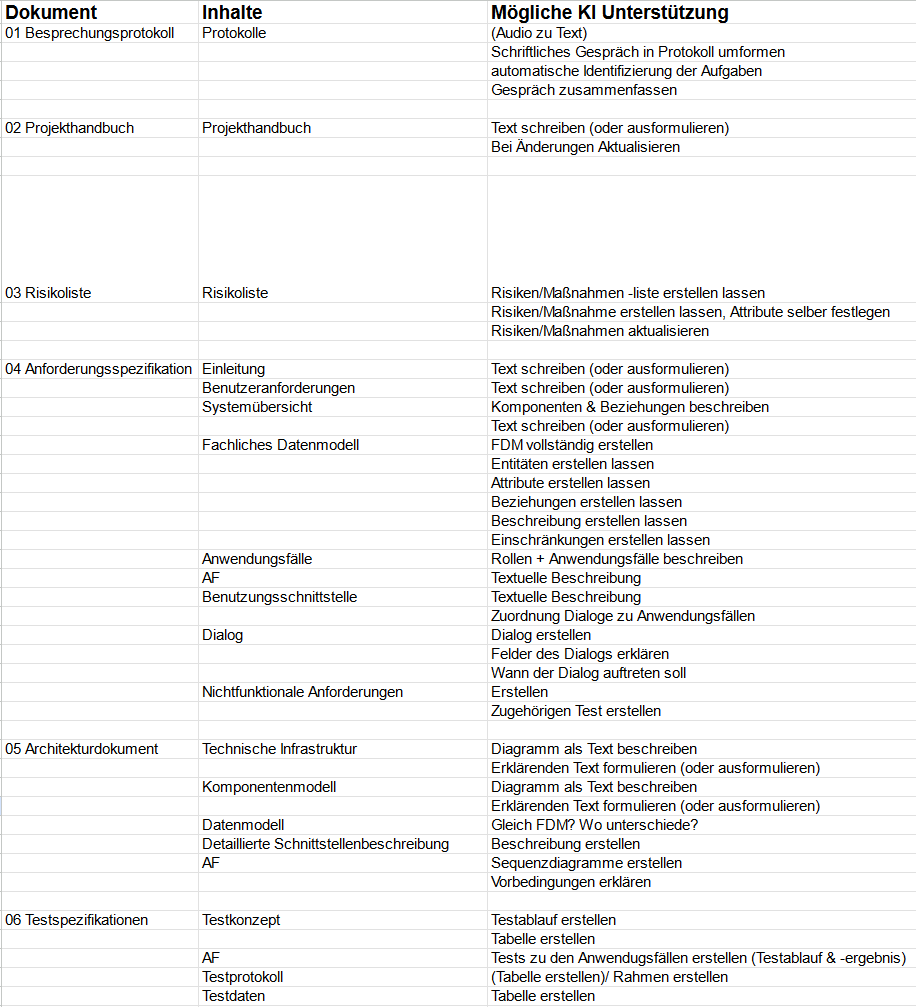
\includegraphics{pictures/Kapitel3Tabelle.PNG}
    \caption{Mögliche LLM Tool Unterstützung}
    \label{Dokumente mit LLM}
\end{figure}

Dieses Kapitel untersucht ausführlich die potenziellen Anwendungsfälle von LLM-Tools im Software Engineering. Dabei 
wird jedes Dokument einzeln betrachtet und aufgezeigt, wie LLM-Tools bei der Erstellung und Verwaltung dieser 
Dokumente eingesetzt werden können. Die \autoref{Dokumente mit LLM} bietet eine Übersicht darüber, in welchen 
Dokumenten und bei welchen Inhalten LLM-Tools unterstützend eingesetzt werden können.

\section{Besprechungsprotokoll} \index{Besprechungsprotokoll} \label{LLMBesprechungsprotokoll}

Im \autoref{Besprechungsprotokoll} wurde bereits erläutert, welche Inhalte in einem Besprechungsprotokoll enthalten 
sind. Nun stellt sich die Frage, wie LLM-Tools bei der Erstellung eines solchen Dokuments unterstützen können.\\

Eine Möglichkeit wäre, das Besprechungsprotokoll aufzeichnen zu lassen und anschließend automatisch daraus das Protokoll 
erstellen zu lassen. Da aktuell jedoch nur die kostenfreie Version ChatGPT-4o mit Dokumenten arbeiten kann, ist dies 
nur in begrenztem Umfang und ohne Vergleiche testbar.\\


Eine weitere Möglichkeit ist es, das Meeting zu verschriftlichen und damit als Texteingabe zu arbeiten. Mit dem 
schriftlichen Gespräch könnten die Tools dann automatisch das Besprechungsprotokoll erstellen.\\
Sollte dies nicht möglich sein, könnte man versuchen, sich die Aufgaben aus dem Gespräch zusammenfassen zu lassen.
Dadurch wäre es einfacher, das Besprechungsprotokoll selbst zu erstellen.\\
Falls auch dies nicht funktioniert, kann das Gespräch zusammengefasst und um unwichtige Themen, wie etwa Abschweifungen, 
gekürzt werden.

\section{Projekthandbuch} \index{Projekthandbuch} \label{LLMProjekthandbuch}

Das Projekthandbuch ist ein zentrales Dokument im Software Engineering Prozess, das alle wesentlichen Informationen und 
Richtlinien eines Projekts zusammenfasst. Die spezifischen Inhalte dieses Dokuments wurden bereits im 
\autoref{Projekthandbuch} dargelegt. Doch wie können LLM-Tools bei der Erstellung des 
Projekthandbuches unterstützend wirken?\\

Eine Möglichkeit besteht darin, das gesamte Projekthandbuch oder einzelne Kapitel von diesen Tools erstellen zu 
lassen. Dafür benötigen die Tools jedoch die relevanten Informationen. Um die Kapitel präziser zu gestalten, könnte 
man diese zunächst in Form von Stichpunkten vorschreiben und anschließend von den LLM-Tools in ausformulierte Texte 
umwandeln lassen.\\
Dabei sollte man sich überlegen, ob es sinnvoll ist, bestimmte Kapitel automatisiert erstellen zu lassen. Ein Beispiel 
hierfür ist die Projektorganisation. In diesem Kapitel werden der Teamaufbau mit den Namen, Rollen und Erreichbarkeiten 
der einzelnen Teammitglieder dokumentiert. In diesem Fall würde es länger dauern, den Prompt für die automatisierte 
Erstellung zu schreiben, als die Daten selbst in die Tabelle einzutragen.\\

Ein weiterer unterstützender Ansatz wäre, dass das Projekthandbuch bei Änderungen, wie beispielsweise personellen 
Veränderungen, automatisch aktualisiert wird.

\section{Risikoliste} \index{Risikoliste} \label{LLMRisikoliste}

Nachdem im \autoref{Risikoliste} die Bestandteile der Risikoliste beschrieben wurden, stellt sich auch hier die Frage, 
wie LLM Tools bei der Erstellung und Pflege der Risikoliste mitwirken und unterstützen können.\\

Eine erste Möglichkeit besteht darin, die gesamte Risikoliste einschließlich der zugehörigen Maßnahmentabelle von 
LLM Tools erstellen zu lassen. Dabei sollten alle Attribute für die Risiken festgelegt werden. Die Werte der einzelnen 
Risikoattribute sollten zudem zueinander in einem konsistenten Verhältnis stehen.\\
Falls dies nicht möglich ist, können LLM-Tools zur Erstellung von Risiken und Maßnahmen herangezogen werden, während 
die Festlegung der Attribute manuell erfolgt.\\

Eine weitere Möglichkeit, wie LLM-Tools bei der Risikoliste unterstützen können, liegt in der Pflege der Liste. Die 
Tools könnten zu bestimmten Zeitpunkten während des Projekts abgefragt werden, ob und wie sich die Risikoliste 
verändert hat. Sollten sich der Status oder andere Attribute der Risiken verändert haben oder sollten Risiken 
eingetreten sein, können die Tools die Risikoliste entsprechend aktualisieren.

\section{Anforderungsspezifikation} \index{Anforderungsspezifikation} \label{LLMAnforderungsspezifikation}

Das \autoref{Anforderungsspezifikation} beschreibt die einzelnen Inhalte der Anforderungsspezifikation. Doch wie 
können LLM-Tools bei der Erstellung dieser unterstützen?\\

Zunächst könnte die Einleitung des Dokuments entweder komplett oder kapitelweise automatisch erstellt werden. Da der 
Kontext hierbei jedoch entscheidend ist, wäre es vermutlich sinnvoller, die Kapitel in Stichpunkten selbst zu 
verfassen und diese dann von den LLM-Tools in zusammenhängende Texte umwandeln zu lassen.\\

Im nächsten Schritt folgen die Benutzeranforderungen. Auch hier besteht die Möglichkeit, den gesamten Text von den 
Tools erstellen zu lassen oder, um eine präzisere Formulierung zu erreichen, die Inhalte zunächst in Stichpunkten zu 
notieren und diese dann ausformulieren zu lassen.\\

Danach kommt die Systemübersicht. Da außer ChatGPT-4o keiner der Chatbots eigenständig Dokumente erstellen kann, 
muss die Zeichnung manuell erstellt werden. Es ist jedoch möglich, die Beschreibung der Komponenten und deren 
Beziehungen von den Tools erstellen zu lassen und diese Beschreibung dann in eine Zeichnung umzusetzen. Ebenso 
kann der Text, der das System beschreibt und in die Systemlandschaft einordnet, automatisch generiert werden. Auch 
hier kann es hilfreich sein, vorab Stichpunkte zu erstellen und diese dann in einen flüssigen Text umwandeln zu lassen.\\

Ähnlich verhält es sich beim fachlichen Datenmodell. Die kostenfreien LLM-Tools können zwar kein UML-Diagramm erstellen, 
aber sie können die Entitäten sowie deren Attribute und Beziehungen beschreiben. Die Diagrammerstellung muss daher 
manuell erfolgen. Die dazugehörigen Beschreibungen und Einschränkungen können hingegen von den Tools generiert werden. 
Falls dies nicht zufriedenstellend funktioniert, können die einzelnen Inhalte wie Entitäten, Attribute, Beziehungen 
sowie Beschreibungen und Einschränkungen jeweils nacheinander separat erstellt werden.\\

Anschließend folgt das Anwendungsfalldiagramm und eine detaillierte Beschreibung der einzelnen Anwendungsfälle mit 
Aktivitätsdiagramm. Das Anwendungsfalldiagramm muss wieder manuell erstellt werden, jedoch können die LLM-Tools 
die Rollen, deren Verbindungen und die zugehörigen Anwendungsfälle auflisten. Falls zusätzliche Bemerkungen zu den 
Anwendungsfällen erforderlich sind, können diese auch von den Tools erstellt werden. Das Aktivitätsdiagramm für die 
Anwendungsfälle muss ebenfalls manuell erstellt werden, wobei eine genaue und detaillierte Beschreibung erforderlich 
ist. Die Beschreibung des Anwendungsfalls kann hingegen vollständig von den Tools generiert werden.\\

Darauf folgt die Benutzungsschnittstelle, die ebenfalls aus einem Diagramm besteht, das zeigt, von welchem Dialog aus 
man zu anderen navigieren kann. Hier kann lediglich eine textuelle Beschreibung von den Tools erstellt werden, während 
das Diagramm manuell erstellt werden muss. Zusätzliche Bemerkungen und die Zuordnung der Dialoge zu den Anwendungsfällen 
können ebenfalls von den LLM-Tools übernommen werden. Die einzelnen Dialoge können textuell beschrieben werden, wobei 
die Tools die einzelnen Eingabefelder und Buttons erläutern sowie definieren können, wann der Dialog aufgerufen wird 
und was beim Schließen des Dialogs passiert.\\

Zuletzt werden die nichtfunktionalen Anforderungen mitsamt den dazugehörigen Tests aufgelistet. Die Anforderungen 
können von den Tools basierend auf den vorherigen Dokumenten erstellt werden. Falls die Tools die Anforderungen nicht 
eigenständig erstellen können, sollten zumindest die Tests von ihnen aufgestellt werden können.

\section{Architekturdokument} \index{Architekturdokument} \label{LLMArchitekturdokument}

Das Architekturdokument beschreibt die grundlegende Struktur und die Designentscheidungen eines Softwareprojekts. 
Die genauen Inhalte wurden bereits im \autoref{Architekturdokument} erläutert. Doch wie können LLM-Tools bei der 
Erstellung dieses Dokuments unterstützen?\\

Die technische Infrastruktur besteht aus einer Grafik und einem erklärenden Text. Bei der Erstellung der Grafik 
stellt sich das Problem, dass nur ChatGPT-4o in der Lage ist, Grafiken zu generieren. Daher muss man sich die 
einzelnen Hardwarekomponenten mit den entsprechenden Versionen und deren Beziehungen zueinander beschreiben lassen 
und die Grafik selbst erstellen. Den dazugehörigen erklärenden Text kann man automatisch generieren lassen. Falls 
dieser nicht präzise genug formuliert ist, kann es hilfreich sein, den Text zunächst in Stichpunkten vorzuschreiben 
und anschließend ausformulieren zu lassen.\\

Anschließend folgt das Komponentenmodell. Auch dieses kann nicht grafisch erstellt werden; lediglich die Komponenten 
und deren Schnittstellen zueinander können definiert werden. Hierzu gibt es einen begleitenden Text, der die 
Komponenten und Schnittstellen beschreibt und deren Funktion erläutert. Dieser Text kann ebenfalls vollständig 
generiert oder in Stichpunkten vorgeschrieben und anschließend ausformuliert werden.\\

Das Datenmodell entspricht häufig dem fachlichen Datenmodell. Hier kann überprüft werden, ob dies der Fall ist und, 
falls nicht, wo die Unterschiede liegen bzw. wie das Datenmodell tatsächlich aussieht.\\

Danach folgt die detaillierte Schnittstellenbeschreibung. Diese ist abhängig von der Projektstruktur der 
Implementierung. LLM-Tools könnten basierend auf den vorherigen Dokumenten eine Projektstruktur erstellen und 
anschließend die Schnittstellenbeschreibung generieren. Wenn jedoch bereits ein Verzeichnis mit den passenden 
Ordnern existiert, sollte die Schnittstellenbeschreibung manuell durchgeführt werden.\\

Nach der Schnittstellenbeschreibung folgt die dynamische Beschreibung exemplarischer Anwendungsfälle. Diese besteht 
aus einem Sequenzdiagramm und den für den Anwendungsfall benötigten Vorbedingungen. Das Sequenzdiagramm kann nur als 
Text beschrieben werden und muss anschließend selbstständig erstellt werden. Die Vorbedingungen sollten ohne 
Schwierigkeiten generiert werden können.

\section{Testspezifikation} \index{Testspezifikation} \label{LLMTestspezifikation}

Im \autoref{Testspezifikation} wurde bereits erklärt, welche Inhalte die Testspezifikation umfasst. Doch wie können 
LLM-Tools bei der Erstellung dieses Dokuments unterstützen?

Zunächst kommt das Testkonzept. Dieses kann automatisch generiert werden. Falls das generierte Konzept nicht den 
eigenen Vorstellungen entspricht, kann man zunächst Stichpunkte selbst schreiben und sich dann den Text daraus 
erstellen lassen. Auch die dazugehörige Tabelle sollte sich von den LLM-Tools erstellen lassen.\\

Anschließend folgen die Tests für die einzelnen Anwendungsfälle. Die Testfälle kann man vollständig von den Tools 
erstellen lassen. Die Testdaten, die bei diesen Tests benötigt werden, werden in einer Tabelle zusammengefasst. 
Auch diese Tabelle könnten die Tools automatisch generieren.\\

Der Rahmen der Tabelle mit dem Testprotokoll kann ebenfalls von den LLM-Tools erstellt werden. Die Ergebnisse 
könnten die Tools auch generieren; allerdings stellt sich hier die Frage, ob dies zu einer Zeitersparnis oder 
einer Arbeitserleichterung führt.\\